\documentclass{article}
\usepackage{graphicx} 
\usepackage[a4paper, margin=2.5cm]{geometry}
\usepackage{minted}
\usepackage{mdframed}
\begin{document}

\title{Hausaufgaben Lösung}
\author{Daniel Schicker}
\date{\today}

\maketitle

\section*{1. Interpreter vs Compiler}
\textbf{Interpretierte Sprachen:}
\begin{itemize}
    \item Der Code wird zur Laufzeit Zeile für Zeile von einem Interpreter gelesen und ausgeführt.
    \item Änderungen am Code können sofort gesehen werden, ohne dass der Code neu kompiliert werden muss.
\end{itemize}

\textbf{Kompilierte Sprachen:}
\begin{itemize}
    \item Der Code wird vor der Ausführung vollständig in Maschinencode übersetzt.
    \item Kompilierte Programme laufen in der Regel schneller, da sie direkt in Maschinencode übersetzt werden.
    \item Änderungen am Code erfordern eine erneute Kompilierung.
\end{itemize}
% Füge hier deine Lösung für Aufgabe 1 ein

\section*{2. Ergebnisse von den 3 Dateien}
\begin{figure}[h]
    \raggedright\caption{Ausführung von Script 1}%
    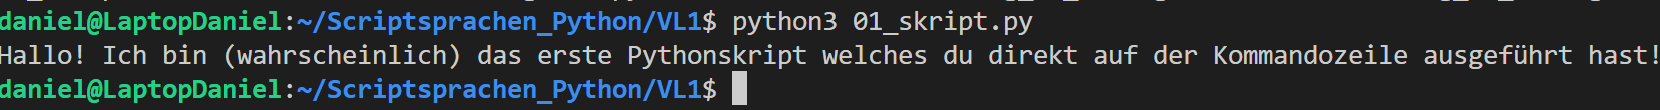
\includegraphics[width=1\textwidth]{ausfuehrung_script1.png}
\end{figure}

\begin{figure}[h]
    \raggedright\caption{Ausführung von Script 2}
    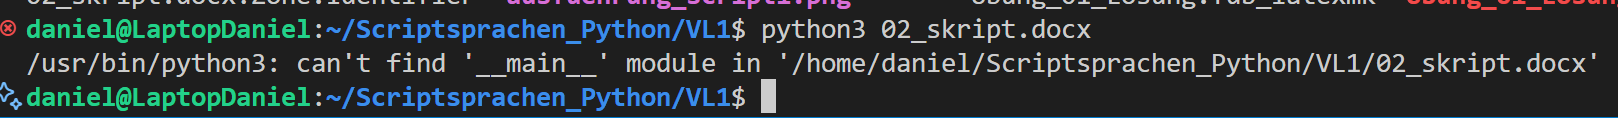
\includegraphics[width=1\textwidth]{ausfuehrung_skript2.png}
\end{figure}

\begin{figure}[h]
    \raggedright\caption{Ausführung von Script 3}
    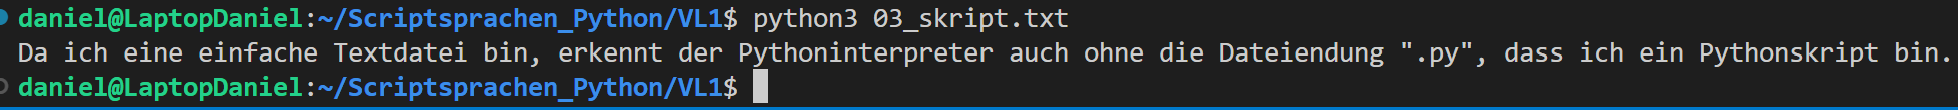
\includegraphics[width=1\textwidth]{ausfuehrung_skript3.png}
\end{figure}

$\Rightarrow$Man erkennt, dass Skript 1 und Skript 3 ausgeführt werden, aber nicht Skript 2, da der Interpreter
\hspace*{2.5em}nicht erkennt, dass es Python Code ist.
\\\\\\\\\\\\\\\\\\\\
\section*{3. Tabellenauswertung}
\begin{table}[h]
    \begin{minipage}{0.5\textwidth}
        \centering
        \begin{tabular}{|c|c|c|c|}\hline
            \textbf{Anweisung} & \textbf{x} & \textbf{y} & \textbf{z} \\
            \hline
            $x = y = 1$ & 1 & 1 & -\\
            \hline
            $x = 2$ & 2 & 1 & - \\
            \hline
            $z = 2 \times 3$ & 2 & 1 & 6\\
            \hline
            $x, y = 1.6$ & error & error & error\\
            \hline
            $sy = 6/2$& 2 & 1 & 6 \\
            \hline
            $z,x = 3.0,6$& 6& 1 & 3.0 \\
            \hline
            $x = "y"$& y & 2 & 3.0 \\
            \hline
        \end{tabular}
    \end{minipage}
    \begin{minipage}{0.5\textwidth}
        \begin{mdframed}[linewidth=1pt, 
            linecolor=black, 
            innerleftmargin=-20pt, 
            innerrightmargin=30pt, 
            innertopmargin=20pt, 
            innerbottommargin=20pt, 
            userdefinedwidth=\textwidth, 
            align=center]
        \begin{minted}{python}
        z = "-"
        x = y = 1
        x=2
        print('x =', x, 'y =', y, 'z =', z)
        z = 2*3
        print('x =', x, 'y =', y, 'z =', z)
        try:
            x,y = 1.6
        except:
            print('fehler bei x,y =1.6')
        sy = 6/2
        print('x =', x, 'y =', y, 'z =', z)
        z,x = 3.0,6
        print('x =', x, 'y =', y, 'z =', z)
        x = "y"
        print('x =', x, 'y =', y, 'z =', z)
        \end{minted}
        \end{mdframed}
    \end{minipage}
\end{table}
\section*{4. Weitere Datentypen}

\begin{itemize}
    \item \textbf{Float:} Eine Gleitkommazahl, die eine Dezimalzahl darstellt.
    \item \textbf{Bool:} Ein boolescher Wert, der entweder wahr oder falsch ist. 
    \item \textbf{char:} Ein einzelnes Zeichen, das in einfachen Anführungszeichen steht.
    \item \textbf{Liste:} Eine Liste ist eine geordnete Sammlung von Elementen, die durch ein Komma getrennt sind und in eckigen Klammern stehen.
    \item \textbf{Tupel:} Ein Tupel ist eine geordnete Sammlung von Elementen, die durch ein Komma getrennt sind und in runden Klammern stehen.
    \item \textbf{Dictionary:} Ein Dictionary ist eine ungeordnete Sammlung von Elementen, die durch ein Komma getrennt sind und in geschweiften Klammern stehen.
\end{itemize}
% Füge weitere Aufgabenlösungen hier hinzu

\end{document}